\chapter{System architecture}
\label{sec:architecture}
\thispagestyle{fancy}
The system is designed around three major data structures, or indices. These are the occurrence index which store inverted lists with positions. The content index stores the content of the documents, and is used for snippets and clustering. The last index is the statistics index which is used to store document statistics which may be used to calculate relevance. 

All these indices are wrapped by one class \texttt{SearchEngineMaster}. The external interface for the system uses this master class to feed documents and to execute queries.  

\section{Statistics index structure}\label{sub:statistics_index_structure}
The statistics index is a mapping from document id to a statistics object containing information such as most frequent term, document vector $tf*idf$ length and number of unique terms.

\section{Content index structure}\label{sub:content_index_structure}
The content index stores the content of the documents indexed, these documents are stored as lists of tokens. These are the raw tokens of the documents nothing is added or removed. By concatenating any consecutive subsequence of these tokens a section of the original document will be produced. This property are used when extracting snippets.  

\section{Occurrence index structure}\label{sub:occurrence_index_structure}
The occurrence index consists of two parts, the dictionary and the inverted file. The dictionary contains the terms of documents, and a pointer into the inverted file. The inverted file contains the inverted lists for each term in alphabetical order. The inverted list of a term contains the documents occurrences that contain the term sorted on increasing document id. Each document occurrence contains a list the positions within the document where the term occurred. The index structure is shown in Figure~\ref{fig:occ_index_struct}.

\begin{figure}[h!!tb]
	\centering
	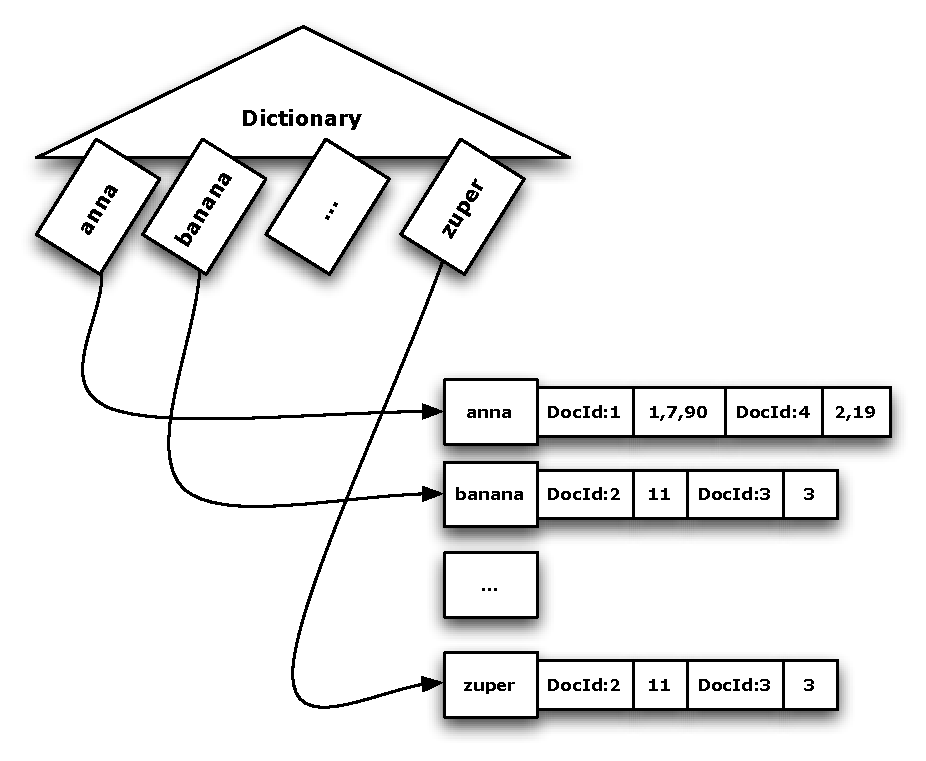
\includegraphics[width=0.8\textwidth]{include/index.pdf}
	\caption[Occurrence index structure]{Occurrence index structure.}\label{fig:occ_index_struct}
\end{figure}

\section{Index building}\label{sub:index_building}
When building indices, all documents fed to the system are given a unique document id from a global counter.

The occurrence index is built in two phases, in the first phase documents are converted to inverted lists and combined into one inverted list representing one index update. 

When the index is flushed, the index update that were built in the first phase is merged with the existing inverted index. Since the inverted lists are sorted on term, document and position merging the lists is a trivial task. 

During this merge, the statistics for each document is calculated and stored in the statistics index. 

When the merge is completed the dictionary is updated so that the pointers in the dictionary points into the newly created inverted file. 

\section{Buffered IO}\label{sec:buffered_io}
One bottleneck of search engines is disk-IO. To use disk-IO as effectively as possible, a buffer manager were designed. The buffer manager splits the files into blocks. When a part of a file is requested for reading or writing it might be buffered. Buffers are managed in a LRU\footnote{LRU: Least Recently Used} fashion. The technicalities of the buffer manager is not deemed interesting in the context of this assignment. 

\section{Feeding pipeline}\label{sec:feeding_pipeline}
The feeding pipeline of our solution is modeled around two main concepts. A document structure which is a object containing various objects with various keys (fields), it's basically a map. A processor is a processing unit in our feeding pipeline which transforms a field in a document structure, and places the result in another. An example of a feeding processor is shown in Figure~\ref{fig:feeding_processor}.

\begin{figure}[htb]
	\centering
	
\includegraphics[width=0.9\textwidth]{include/processor.pdf}
	\caption[Feeding pipeline example]{Feeding pipeline example, a html to text processor strips away html from the input field ``content'', and puts the result into the ``cleaned'' field.}\label{fig:feeding_processor}
\end{figure}

\subsection{Feeding processors}\label{sub:implemented_feeding_processors}
To be able to solve the task the feeding pipeline has to implement multiple feeding processors. These are:

\begin{itemize}
	\item \textbf{HtmlToText:} strips away HTML tags.
	\item \textbf{Tokenizer:} brakes the documents into tokens. These tokens are the raw tokens of the documents, that is, no characters are removed from the text, the text is only split into pieces.
	\item \textbf{PunctuationRemover:} removes punctuations and whitespaces from tokens. 
	\item \textbf{Stemmer:} reduces tokens to their stems. 
	\item \textbf{Termizer:} creates inverted documents, collecting position lists for each term in the document.
\end{itemize}

\section{Query processing}
The query processing part of the system is designed to be both flexible and extensible. The main idea is to have a query processor which uses a query preprocessor and a (number of) query processing components to produce and sort the query results. A query preprocessor uses a number of built-in stages (similar to those used for the document processing) to transform a textual query into a query structure.

A query processing component, on the other hand, is an abstract component that may be used to pull query results. Each component may include another component as a source, and it is possible to construct a chain of such components. To begin with, a minimal number of processing components include:
\begin{itemize}
	\item {\bf Matcher:} produces a number of combined results for a given query. These match inclusion and exclusion of terms based on AND, OR and NAND modifiers.
	\item {\bf Score Combiner:} pulls from its source and scores them according to a number of score modules that can be added to the system. The system may implement a number of different similarity models (both dynamic and static) and a score combiner can calculate a weighted average from these.
	\item {\bf Filters:} may filter out some of the results based on a number of abstract filters that can be later implemented and added to the system.
\end{itemize}

The query processing structure implemented in the initial implementation of solbrille is shown in Figure~\ref{fig:query_processing}.

\begin{figure}[ht]
	\centering
	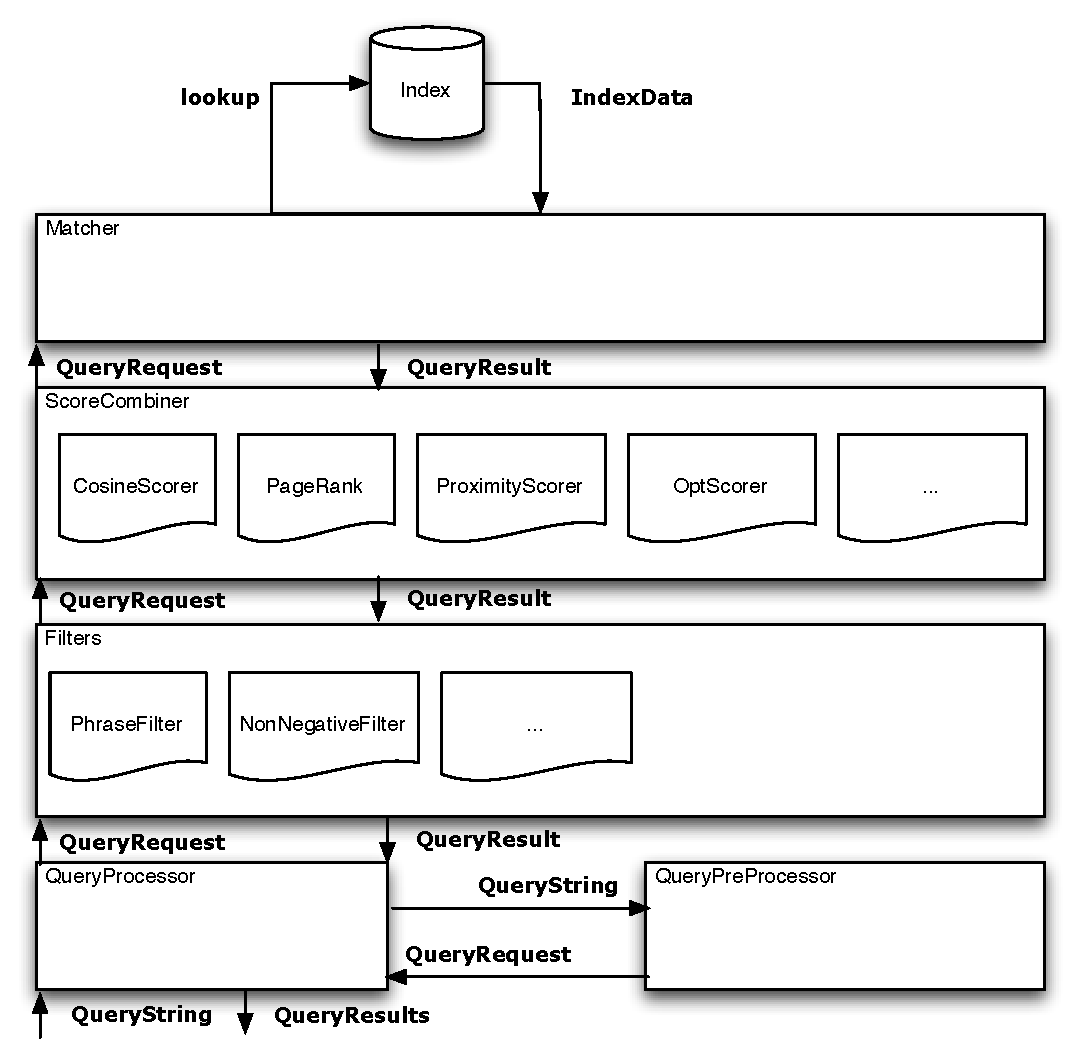
\includegraphics[width=0.9\textwidth]{include/query_processing.pdf}
	\caption{Query processing subsystem.}\label{fig:query_processing}
\end{figure}

The most important point here is that the query processor does not have to know what components are used in the query processing, and a system implementation is free to extend the number of components, add several instances of the same component in the processing pipeline or change the processing order of these. 

In future, the system may be extended by a merger that enables to merge a number of processing pipelines into one. In this case, the system may become distributed. For example, it may run a number of basic matchers, scorers and filters on a number of different nodes, then results from these may be pulled together by a new merger component which may combine the results. If required, the processing pipeline may be extended by a couple of new filters and scorers used to re-weight and filter the combined results. However, due to the project duration limits the target search engine is chosen to run only on a single computer.

The rest of this section explains the basic processing components and the ideas behind.

\subsection{Matcher component}
The matcher component is the part of the processing pipeline which performs the actual lookups into the inverted index (OccurenceIndex). The matcher extracts the various terms referenced in a query and executes one lookup for each of the terms. It also recognizes the modifiers associated with the terms (\emph{AND}, \emph{OR} and \emph{NAND}). The matchers purpose is to create candidate results for further filtering and ranking. A candidate result is a document which satisfies the query. That is, a document where \emph{all} terms with a \emph{AND} modifier is present and \emph{no} terms with a \emph{NAND} modifier. In addition the terms with \emph{OR} modifiers are appended to the documents which satisfies the \emph{AND} and \emph{NAND} requirements.

The matcher component allows us to support a limited subset of boolean queries, however, since it has no aspect of parenthesises the subset is rather small. For vector space queries, all terms are treated with \emph{OR} modifiers.

\subsubsection{Critique and an alternative approach}\label{sssub:matcher_critique}
To support the full range of boolean queries a tree of \emph{AND}, \emph{OR} and \emph{NAND} matching components could have been constructed. This would have been a much more flexible way of building result candidates. Merging all functionality for doing matching into one component  also leads to one piece of very complex code. While implementing the matcher we had quite a few subtile bugs which took us quite some time to figure out. 

The reason we did not use a more general scheme were that index term could have ben looked up multiple times. However, this is not a issue with the proposed design for buffer manager and processing component. Since the results are pulled one by one and combined as soon as possible, a repeated request to the same term will be cached in the buffer manager. Therefore the performance impact of this general scheme is close to nothing. 

\subsection{Score Combiner and Scorer Components}
The idea with score combiner is to retrieve a number of score values from different scorers, and then combine these into a total score. The main intention here is that the system may implement different scoring models or even combine these. A scorer may implement a cosine model, a probabilistic model such as Okapi BM-25, a static link-analysis models such as PageRank or HITS, or even an Opt model\footnote{the optimal model, an inside joke}.

To be fast, some of the document collection statistics later required by scorers has to be stored in the query requests and query results, since the access to global statistics on demand may be too slow. 

\subsection{Filters and Phrase Search}
To demonstrate the idea with filters the system is intended to present two types of filters, a non-negative filter and a phrase filter. A non-negative filter is rather a demonstation of the concept and it can just filter out the results which have a score value less or equal to zero. However, using the scorer components specified above, this situation is impossible.

A phrase filter has a more practical application. The main intention is to filter results based on + and - phrases.

A simple case for the phrase search is either a phrase such as {\it +''kari bremnes''} or a phrase like {\it kari +''kari bremnes''}. The solution for both of these is to represent AND phrases as lists of terms in the query structure, match and score the corresponding terms just as normal terms, and then finally check if these terms occur in the required order using the document occurrence part of the inverted index.

A more problematic case for the phrase search is a query such as {\it kari -''kari bremnes''}. In this case the user wants to retrieve all the documents containing word {\it kari}, but not the word {\it kari} followed by the word {\it bremnes}.

The solution is to introduce a fourth modifier type, PNAND. As for the AND phrases, the query structure has to store a number of phrases represented as a modifier (AND or NAND) and a list of terms. All the terms represented in a phrase has the same modifier as the phrase itself, and terms having both PNAND and an other modifier have to loose the PNAND modifier. The matcher component has to perform a match on both NAND, OR and AND terms, and also PNAND terms interpreted as OR terms. Any scorer component has then to ignore PNAND terms, giving 0 in the score impact of these. Any results matching either NAND phrases of only PNAND terms have to be removed in the phrase filter.

Finally, in the current design a result says to be filtered out if one of the filters does not approve the result. This approach can be later extended to use a boolean expression of filter constraints, represented as a tree or similar.

\subsubsection{Critique and an Alternative Approach}
The approach described above is chosen to be implemented, just to demonstrate the idea behind the filtering component. However, as the phrase filtering is now performed during all the stages of the query processing pipeline this method is rather impractical. A better solution that can be applied in future is to use a separate phrase matcher, and then combine the matched phrase results and the ordinary term results before sending these to a scorer component. The same critique mentioned in Section~\ref{sssub:matcher_critique} with respect to multiple index lookups applies for this as well.

\subsection{Final Details}
To save memory the results pulled by the query processor are stored into a priority queue. As a query is expected to be a query string and a page range {\it startpage} end {\it endpage}, the maximum queue size is limited by {\it endpage}. When the queue size has reached this value a new candidate has to be compared with the least scored result contained in the queue. If the candidates value is greatest of these two, the candidate has to replace the least scored result in the priority queue.

When all the results are processed, up-to {\it endpage} - {\it startpage} results has to be extracted from the queue, sorted in descending order and returned to the user.

\section{Extended System}

\section{Testing and Front-End Design}

